\section{Introduction}
\begin{frame}
  \frametitle{The proof system Coq}
  A language to:
  \begin{itemize}
    \item state theorems
    \item write proofs verified by computer
    \item write algorithms
  \end{itemize}
\end{frame}

\begin{frame}[fragile]
  \frametitle{Raw example}
  \begin{verbatim}
Fixpoint fact (n:nat) : nat :=
  match n with
    | O => 1
    | S n => S n * fact n
  end.

Arguments fact n%nat.

Lemma lt_O_fact n : 0 < fact n.
Proof.
  induction n; simpl; auto with arith.
Qed.
  \end{verbatim}
\end{frame}

\begin{frame}
  \frametitle{The proof system Coq}
  An environment to:
  \begin{itemize}
    \item reason interactively
    \item organize and distribute proofs
  \end{itemize}
\end{frame}

\begin{frame}
  \frametitle{IDE}
  \begin{center}
    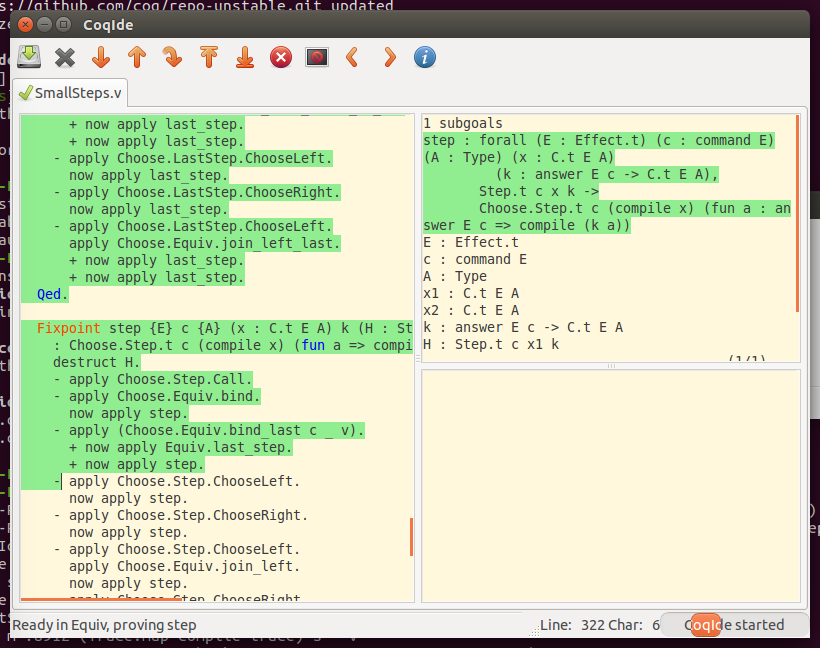
\includegraphics[width=9cm]{images/ide}
  \end{center}
\end{frame}

\begin{frame}
  \frametitle{Distribute}
  \begin{center}
    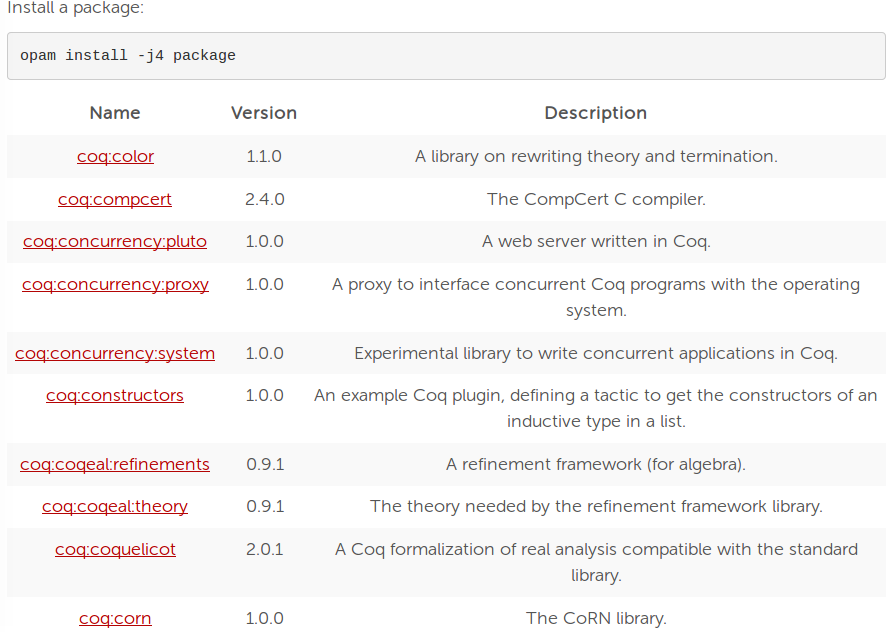
\includegraphics[width=10cm]{images/opam}
  \end{center}
\end{frame}

\begin{frame}
  \frametitle{Usage}
  Maths:
  \begin{itemize}
    \item four colors theorem (Gontier 04)
    \item Feit -- Thompson theorem (odd order theorem) (Gontier \& all, 12)
  \end{itemize}

  Computer sciences:
  \begin{itemize}
    \item certified \textsc{C} compiler CompCert (Xavier Leroy \& all)
    \item \emph{Bedrock} library for low-level programs (Adam Chlipala \& all)
  \end{itemize}

  Many conference papers with Coq proofs in annex.
\end{frame}

% \begin{frame}
%   \frametitle{Historique}
%   \begin{itemize}
%     \item Calcul des Constructions (\textsc{CoC}) par \emph{Thierry Coquand} (85)
%     \item implémentation du \textsc{CoC} donnant lieu à \textsc{Coq}
%     \item Calculus of Inductive Constructions (\textsc{CiC}) par \emph{Christine Paulin} (91)
%   \end{itemize}
% \end{frame}

% \begin{frame}
%   \frametitle{Logique}
%   \begin{itemize}
%     \item théorie des types plutôt que ensembles
%     \item logique intuitionniste et constructive
%     \item axiomes du tiers exclu, du choix optionels
%   \end{itemize}
% \end{frame}
